% !TEX root = ../../../prj4projektdokumentation.tex

\section{Modultest}

\subsection{Kontrolmodul}

\begin{center}
	\begin{tabular}{ | m{0.2\textwidth} | m{0.8\textwidth}|} 
		\hline
		\textbf{Test}					&Opret forbindelse fra en TCP client på PLC'en til en TCP server på en Windows PC. \\ \hline
		\textbf{Testbeskrivelse}		&Funktionen OpretForbindelse i PLC programmet testes ved hjælp af et en test server Winsock!!!!BILAG!!!!. Testen overvåges ved at gå online på PLC'en og gennem udskrifter fra Winsock programmet i en kommandoprompt på PC'en. EnableForbindelse styres af en switch forbundet til indgangen I0.0 i PLC'en.\\ \hline
		\textbf{Input}					& Et on switch på I0.0.\\ \hline
		\textbf{Forventet output}		&Clienten vil være aktiv i at oprette forbindelse, hvilket vil betyde at serveren udskriver at den har nedlagt listen socket og er klar til at modtage data.\\ \hline
		\textbf{Resultat}				&EnableForbindelse bliver sat true og i kommandoprompten udskriver serveren at listen socket er nedlagt og at den er klar til at modtage data. Se figur \ref{fig:OpretForbindelseFoer} og figur \ref{fig:OpretForbindelseEfter}.   \\ \hline
	\end{tabular}
\end{center}

\begin{figure}[H] % (alternativt [H])
	\centering
	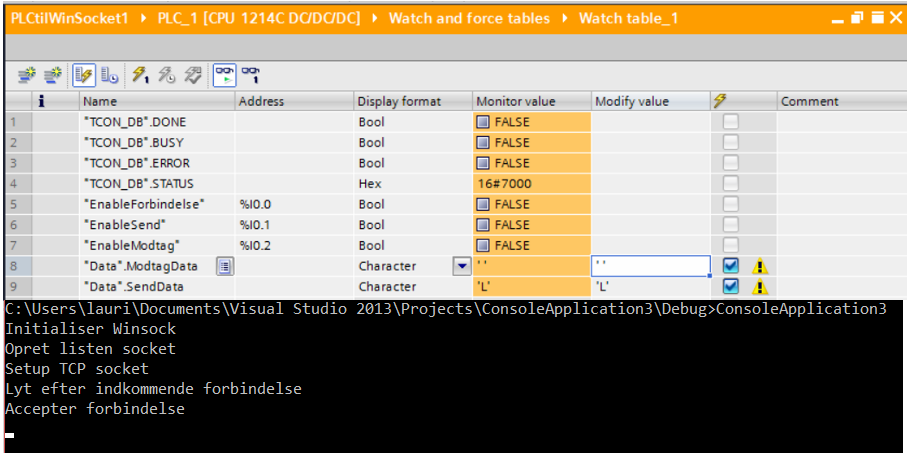
\includegraphics[width=0.85\textwidth]{Test/ModultestStyringsenhed/OpretForbindelseFoer}
	\caption{Før I0.0 swicthes on}
	\label{fig:OpretForbindelseFoer}
\end{figure}

\begin{figure}[H] % (alternativt [H])
	\centering
	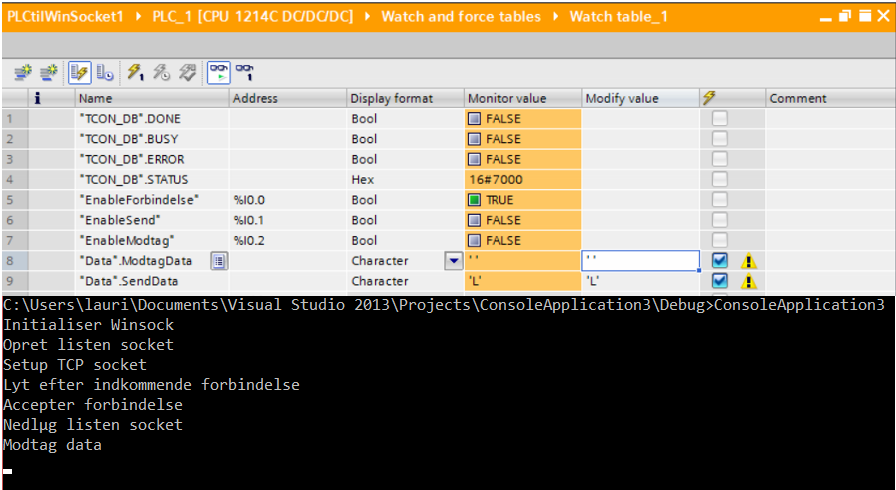
\includegraphics[width=0.85\textwidth]{Test/ModultestStyringsenhed/OpretForbindelseEfter}
	\caption{Ffter I0.0 swicthes on}
	\label{fig:OpretForbindelseEfter}
\end{figure}

\begin{center}
	\begin{tabular}{ | m{0.2\textwidth} | m{0.8\textwidth}|} 
		\hline
		\textbf{Test}					&Send data fra en TCP client på PLC'en til en TCP server på en Windows PC. Samme data sendes retur fra server til client. \\ \hline
		\textbf{Testbeskrivelse}		&Funktionerne SendData og ModtagData i PLC programmet testes ved hjælp af et en test server Winsock!!!!BILAG!!!!. Testen overvåges ved at gå online på PLC'en og gennem udskrifter fra Winsock programmet i en kommandoprompt på PC'en. EnableSend og EnableModtag styres af to switches forbundet til indgangene I0.1 og I0.2. \\ \hline
		\textbf{Input}					& Et on switch på I0.0, I0.1 og I0.2.\\ \hline
		\textbf{Forventet output}		&Char arrayet 'A', 'B', 'C', 'D' vil blive sendt og modtaget igen. Det kan ses på udskrifter at i kommandoprompten at 4 bytes er modtaget og sendt igen, hvorefter serveren er klar til at modtag ny data. På PLC'en kan det ses at de 4 sendte bytes matcher de 4 modtagne.\\ \hline
		\textbf{Resultat}				&EnableForbindelse, EnableSend og EnableModtag bliver sat true og i kommandoprompten udskriver serveren at 4 bytes er modtaget og 4 er bytes er sendt og at den er klar til at ny modtage data. PLC'en har de samme 4 bytes i ModtagDat arrayet som i SendData arrayet. Se figur \ref{fig:ModtagDataOgSendData} \\ \hline
	\end{tabular}
\end{center}

\begin{figure}[H] % (alternativt [H])
	\centering
	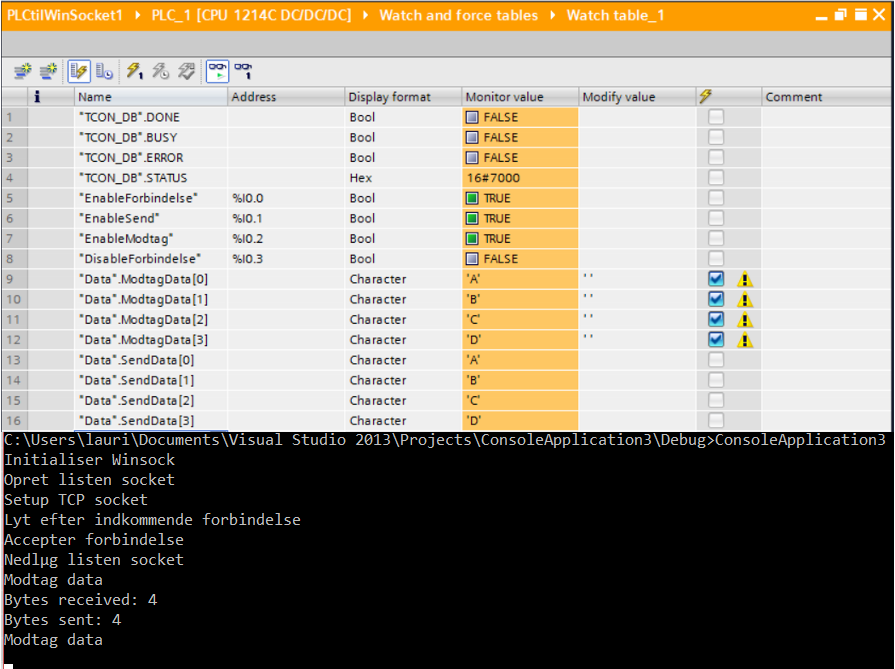
\includegraphics[width=0.85\textwidth]{Test/ModultestStyringsenhed/ModtagDataOgSendData}
	\caption{Test af ModtagData og SendData}
	\label{fig:ModtagDataOgSendData}
\end{figure}

\begin{center}
	\begin{tabular}{ | m{0.2\textwidth} | m{0.8\textwidth}|} 
		\hline
		\textbf{Test}					&Nedlæg forbindelsen mellem en PLC client og en Windows server.\\ \hline
		\textbf{Testbeskrivelse}		&Funktionen AfslutForbindelse i PLC programmet testes ved hjælp af en test server Winsock !!!BILAG!!!. Testen overvåges ved at gå online på PLC'en og gennem udskrifter fra Winsock programmet i en kommandoprompt på PC'en. DisbaleForbindelse styres af to swicthes forbundet til indgangen I0.3. \\ \hline
		\textbf{Input}					& Et on switch på I0.3\\ \hline
		\textbf{Forventet output}		&Winsock programmet vil udskrive en fejl, fordi det har mistet forbindelsen. \\ \hline
		\textbf{Resultat}				&DisableForbindelse bliver sat true og i kommandoprompten udskriver serveren at der skete en fejl i modtagelse af ny data og udskriver fejlkode. Se figur \ref{fig:AfslutForbindelse} \\ \hline
	\end{tabular}
\end{center}

\begin{figure}[H] % (alternativt [H])
	\centering
	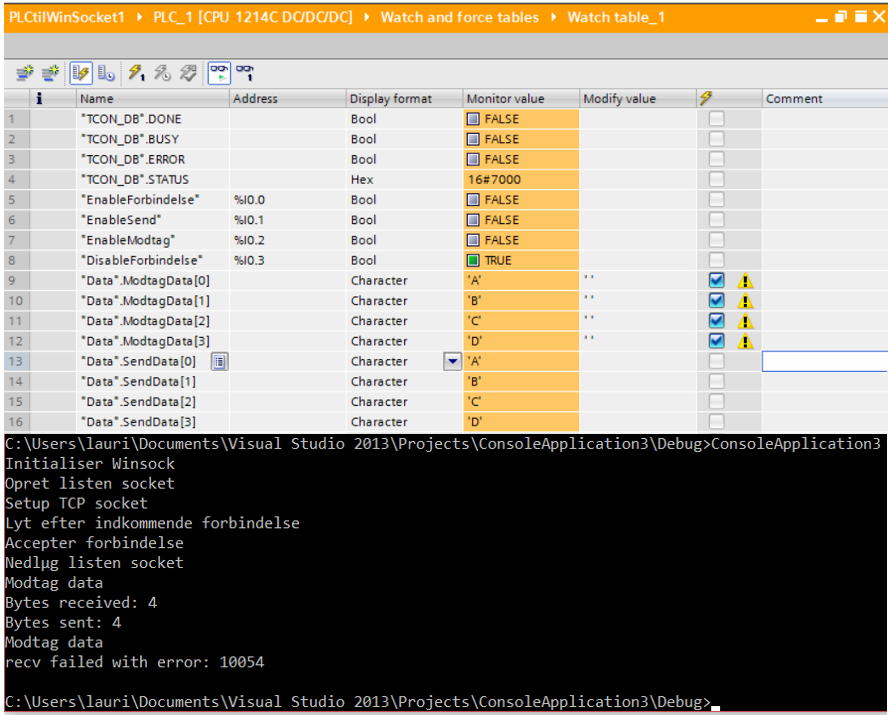
\includegraphics[width=0.85\textwidth]{Test/ModultestStyringsenhed/AfslutForbindelse}
	\caption{Test af AfslutForbindelse}
	\label{fig:AfslutForbindelse}
\end{figure}

\begin{center}
	\begin{tabular}{ | m{0.2\textwidth} | m{0.8\textwidth}|} 
		\hline
		\textbf{Test}					&PLC udgangene til relæer leverer 24V, som skal til for at relæerne slår. \\ \hline
		\textbf{Testbeskrivelse}		&Rælerne der bruges til at styre hvilket transformertrin der benyttes skal have 24V for at slår. Derfor testes det at udgangene også giver 24V.\\ \hline
		\textbf{Input}					& \\ \hline
		\textbf{Forventet output}		&Det forventes at der kan måles 24V med et multimeter.\\ \hline
		\textbf{Resultat}				&Spænding målte på PLC udgang: 24.07 V, 23,97 V, 24.08 V   \\ \hline
	\end{tabular}
\end{center}

\subsection{Brugergrænseflade}

\begin{center}
	\begin{tabular}{ | m{0.2\textwidth} | m{0.8\textwidth}|} 
		\hline
		\textbf{Test}					&HMI'en udskriver random generede tal der sendes til PLC'en fra PSoC'en. \\ \hline
		\textbf{Testbeskrivelse}		&PSoC'en er opsat med en speciel kode se figur \ref{fig:PSoCkodeeksempel}, der genererer tilfældige værdier for strøm, spænding, powerfactor og THD.  \\ \hline
		\textbf{Input}					& Måledata over fra PsoC'en til PLC'en, hvor HMI'en kan hente data fra og vise dem på skærmen.\\ \hline
		\textbf{Forventet output}		&HMI'en opdateres med nye tilfældige værdier kontinuerligt.\\ \hline
		\textbf{Resultat}				&Måleværdierne på skærmen bliver opdateret en gang hver 2s.  !!! MANGLER BILLEDE !!!\\ \hline
	\end{tabular}
\end{center}

\begin{figure}[H] % (alternativt [H])
	\centering
	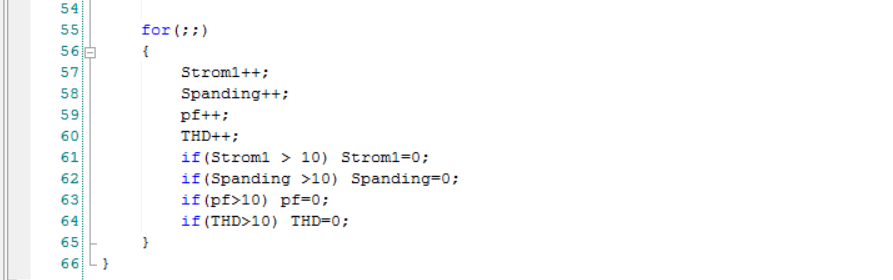
\includegraphics[width=0.85\textwidth]{Test/ModultestStyringsenhed/PSoCkodeeksempel}
	\caption{PSoC tæller op og sender derfor tilfældige data}
	\label{fig:PSoCkodeeksempel}
\end{figure}


\subsection{Kommunikationsmodul}

\begin{center}
	\begin{tabular}{ | m{0.2\textwidth} | m{0.8\textwidth}|} 
		\hline
		\textbf{Test}					&Arduino'en modtager 'req1' over Ethernet fra PLC'en.  \\ \hline
		\textbf{Testbeskrivelse}		&Før Arduino'en sender værdierne til PLC'en skal den modtage et request på de nye værdier, det testes her om Arduinoen med denne request kommando rigtigt.  \\ \hline
		\textbf{Input}					& PLC'en udsender request kommandoen 'req1' over Ethernet.\\ \hline
		\textbf{Forventet output}		&Arduinoen vil udskrive req1 på det serielle vindue, der kan åbnes i udviklingsprogrammet. \\ \hline
		\textbf{Resultat}				&Arduinoen modtager 'req1' og udskriver det på det serielle vindue. Se figur  \ref{fig:RequestModtagelse} \\ \hline
	\end{tabular}
\end{center}

\begin{figure}[H] % (alternativt [H])
	\centering
	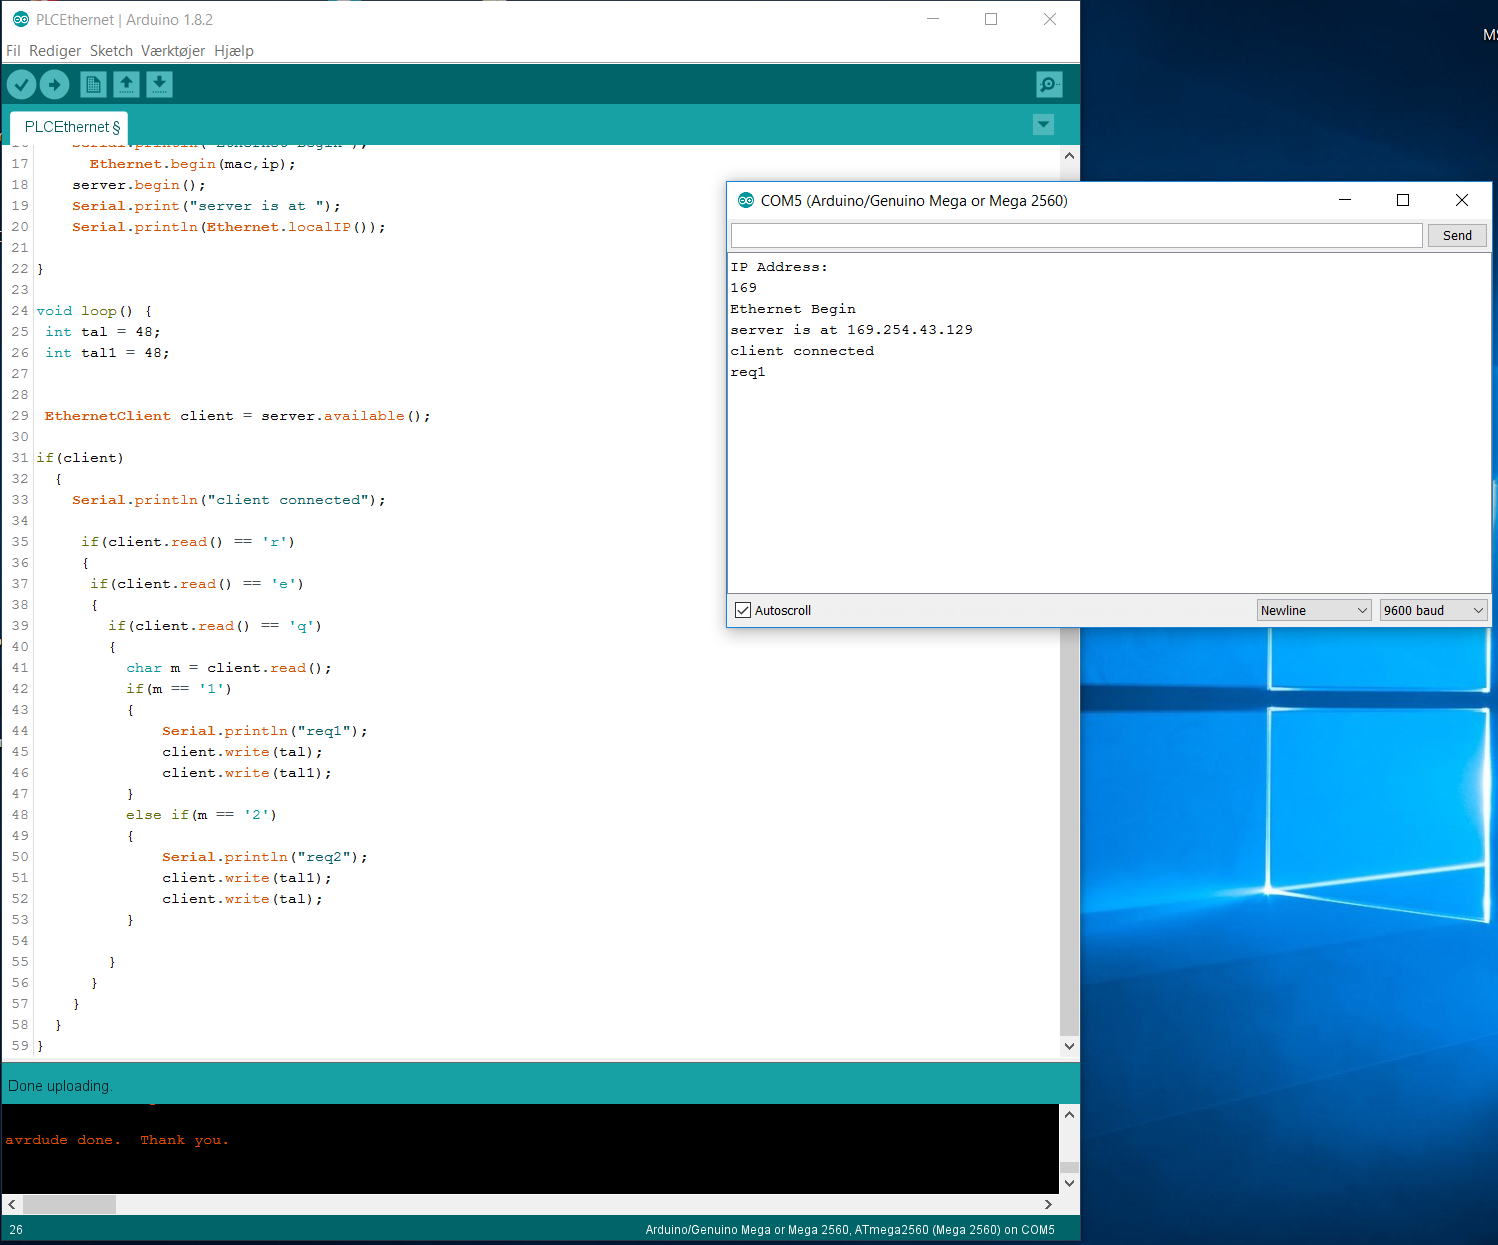
\includegraphics[width=0.85\textwidth]{Test/ModultestStyringsenhed/EthernettestArduinoTerminal}
	\caption{Test af request modtagelse}
	\label{fig:RequestModtagelse}
\end{figure}

\begin{center}
	\begin{tabular}{ | m{0.2\textwidth} | m{0.8\textwidth}|} 
		\hline
		\textbf{Test}					&Arduino'en kan modtage værdi over UART fra PSoC'en.   \\ \hline
		\textbf{Testbeskrivelse}		&Arduino'en skal modtage måledata fra PSoC'en for 4 forskellige målinger. Der bliver holdt styr på hvilke måledata der kommer hvornår, ved at Arduioen efterspørger hver enkelt måledata over UART linjen, med 'A', 'B', 'C' eller 'D'. Dette ses på figur \ref{fig:Hentmaaledata}, hvor Serial.write() skriver til terminal vinduet, og Serial1.write() skriver til PSoC'en. \\ \hline
		\textbf{Input}					& Arduinoen udsender 'A', 'B', 'C' og 'D' i et loop. Der modtages derfor måledata, der tilfældig genereret på PSoC'en.  \\ \hline
		\textbf{Forventet output}		&Arduinoen vil udskrive de modtagede tilfældige måledata på terminalvinduet \\ \hline
		\textbf{Resultat}				&Arduinoen modtager udskriver måledata i terminalvinduet. Se figur \ref{fig:Hentmaaledata} \\ \hline
	\end{tabular}
\end{center}

\begin{figure}[H] % (alternativt [H])
	\centering
	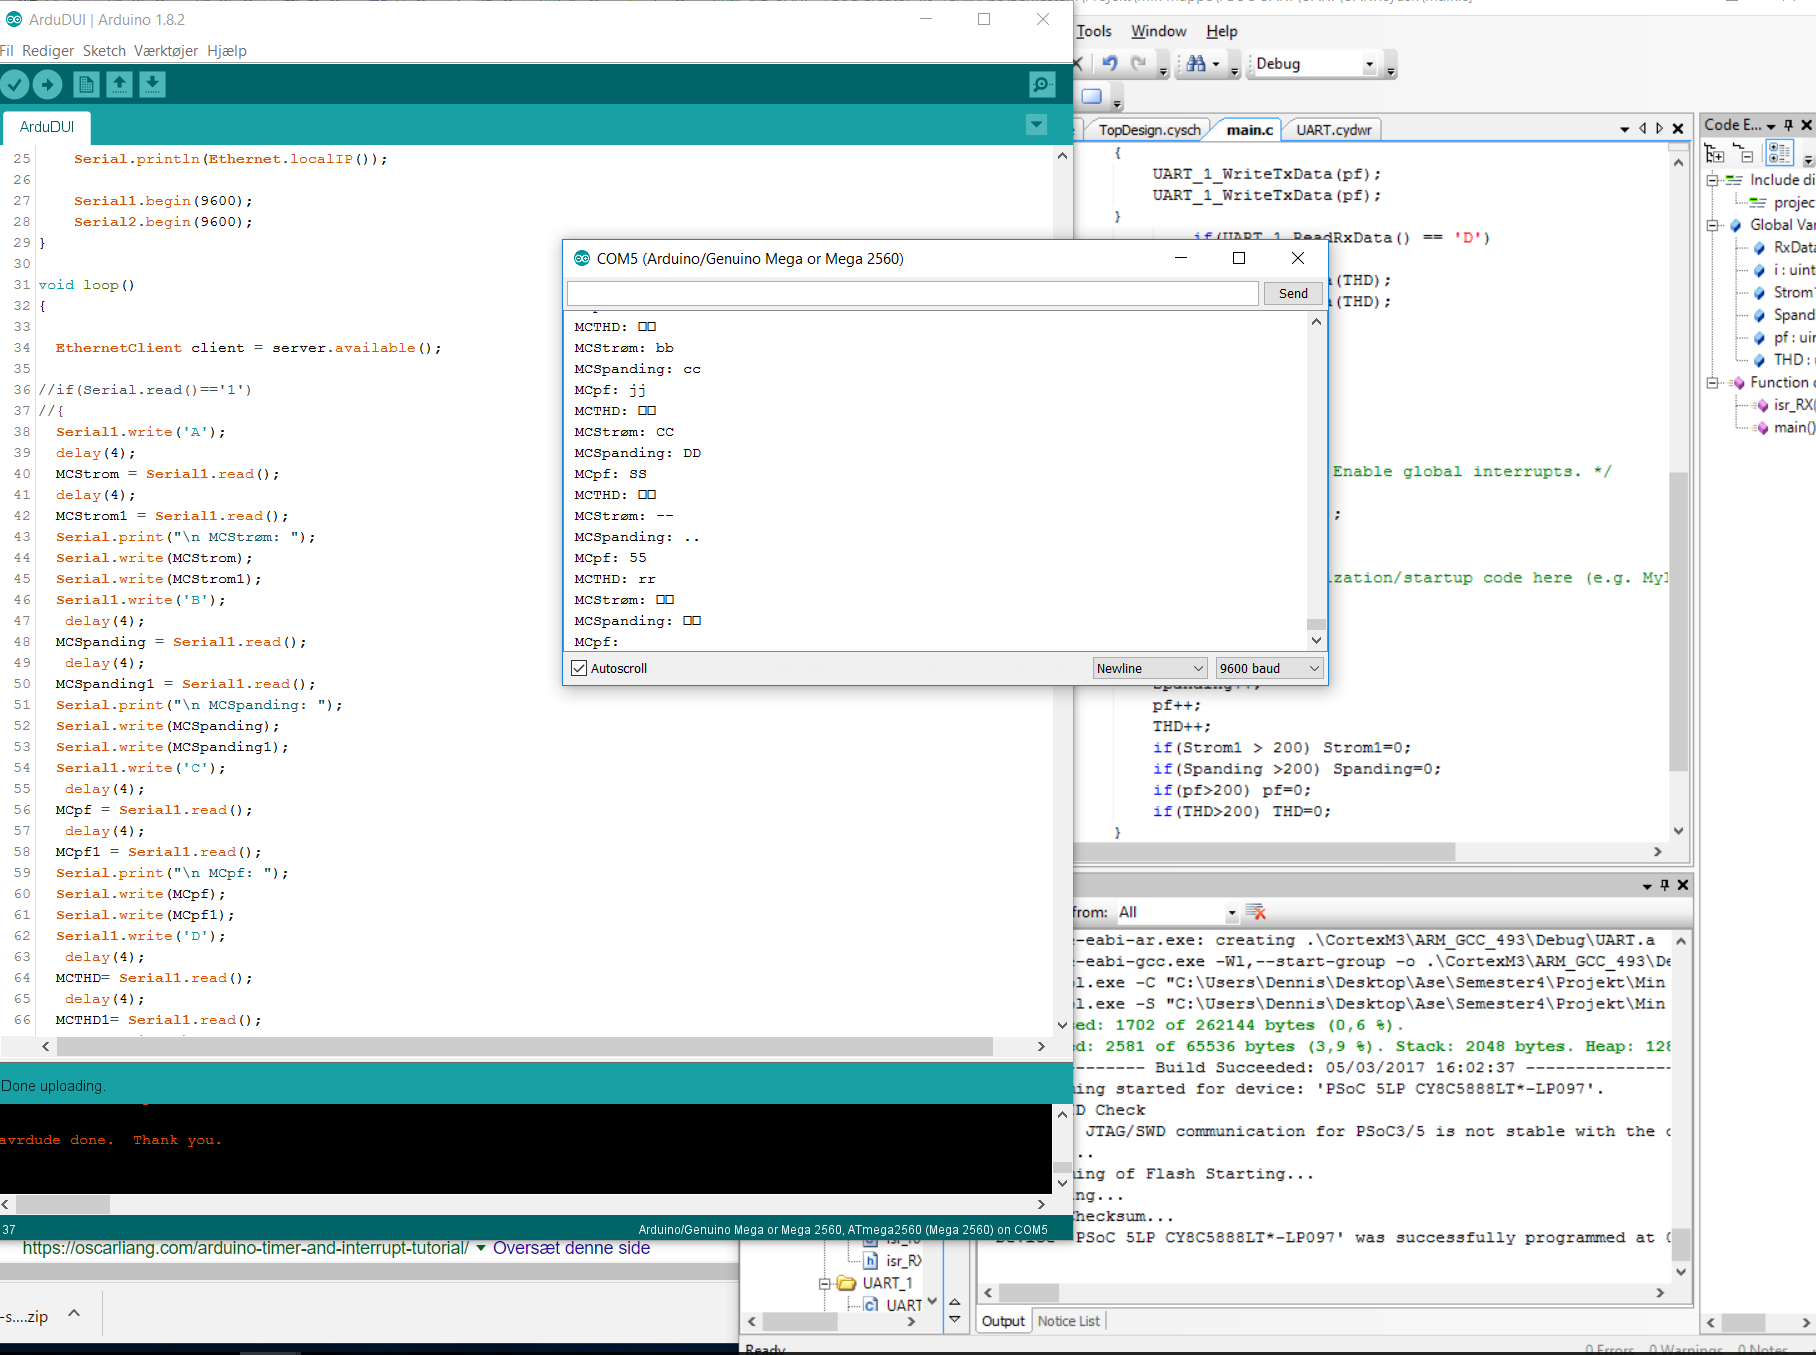
\includegraphics[width=0.85\textwidth]{Test/ModultestStyringsenhed/EthernettestkontinuertDataflow}
	\caption{Test af måledata modtagelse}
	\label{fig:Hentmaaledata}
\end{figure}